\begin{frame}{Trouvons des négatives}
  \begin{enumerate}
    \item Écris trois questions qui pourraient susciter \gloss{elicit} des réponses négatives.
    \item<2-> Pour chaque question, trouve une personne dans la classe qui répond «non», et écris son nom à côté de la question. \emph{Répondez avec des phrases complètes!}
  \end{enumerate}
  \begin{center}
    \footnotesize
    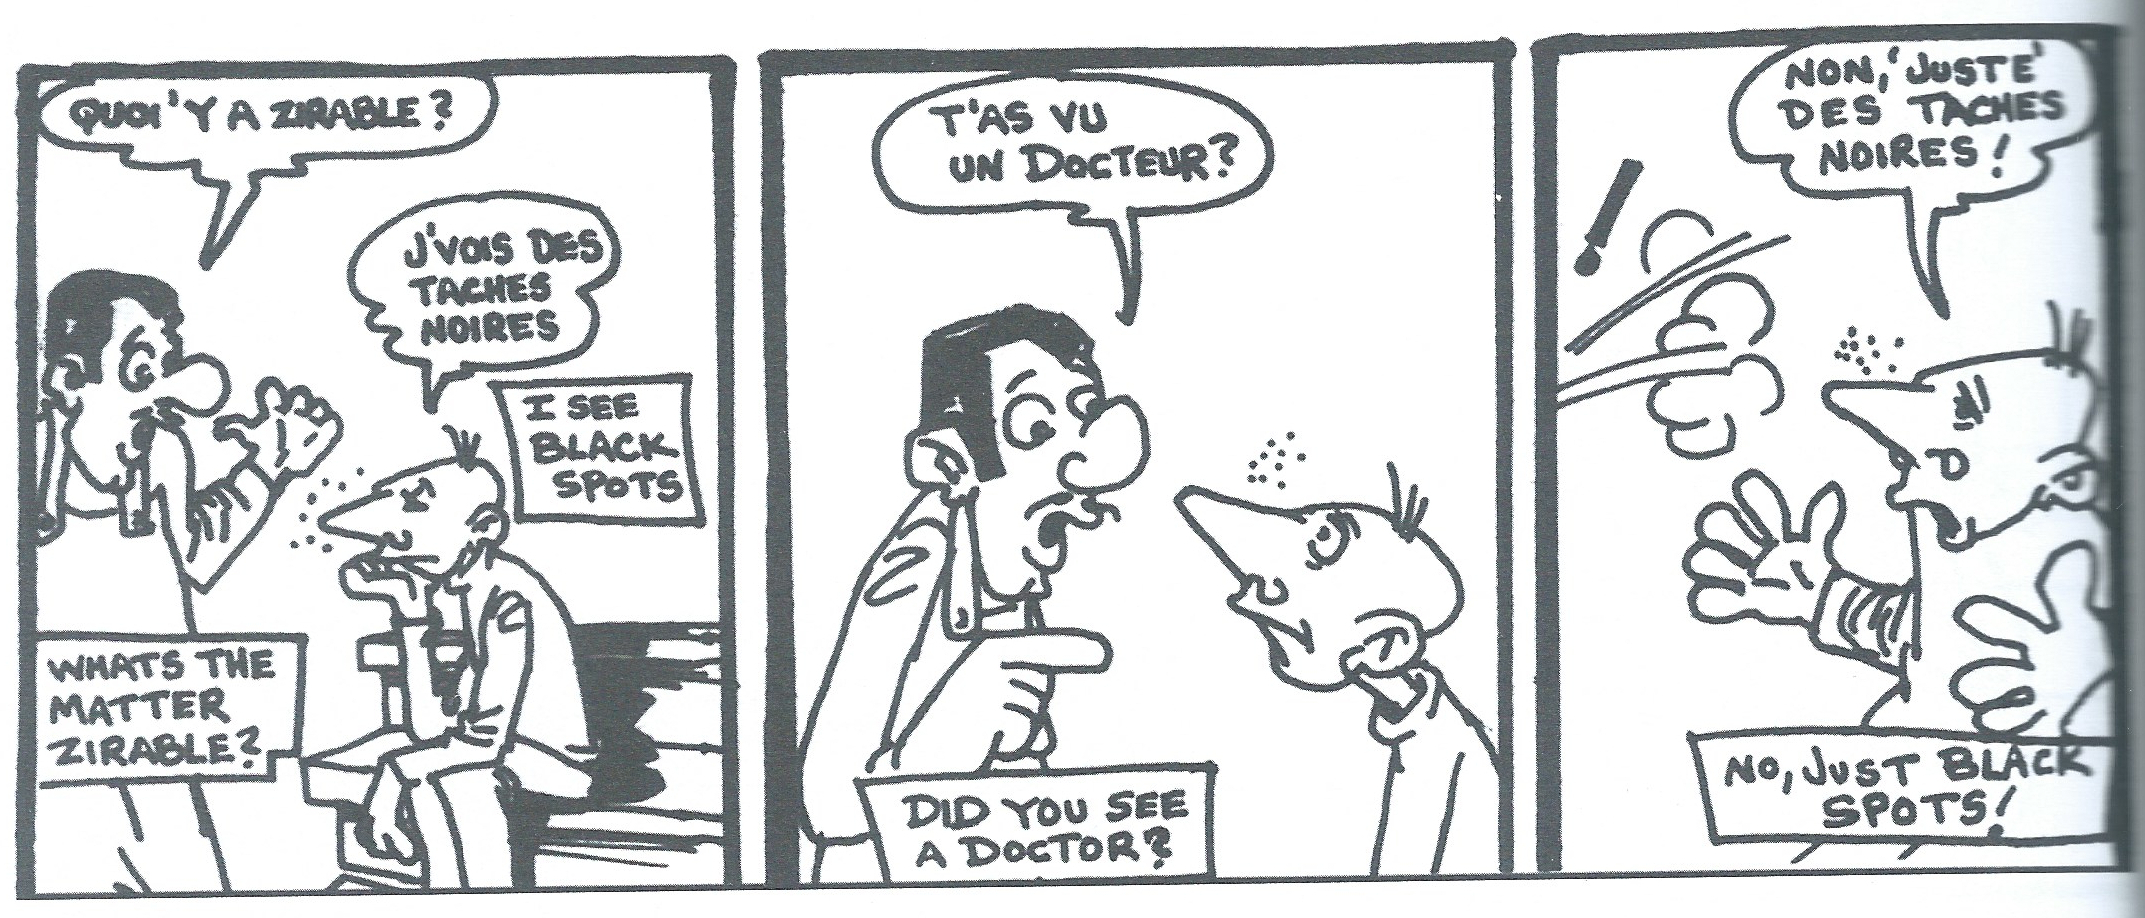
\includegraphics[scale=0.55]{bec_doux.jpeg} \\
    Bec Doux, 1971, bande dessinée de Louisiane
  \end{center}
\end{frame}